\subsection{Supply Chain: Tracking Fish from Ocean to Table}

Oceanic fishing represents more than \$ 100B in economic impact worldwide. In spite of its impact,
the industry is fraught with problems. Estimates suggest that nearly 20\% of fish are caught
illegally. In addition to the environmental impact of illegal fishing, the integrity of the industry
is also affected; a recent study based on DNA testing found that nearly $\frac{1}{3}$ of all fish
was mislabeled including 87\% of snapper and 57\% of tuna (95\% of all sushi restaurants were found
to serve mislabeled fish).

Traceability and provenance are managed in several limited domains such as Maine lobster and
Maryland crab. However, the complexity of the ecosystem (see the figure below) and its relatively
primitive use of technology limit the impact (see this article for more information on efforts to
enable traceability more broadly). Problems identified by FishWise in a 2012 study include:

Many different paths from ocean to table Lake of global authority for tracing Existing proprietary
tracing systems unscalable Most existing processes are paper-based

Oceana postulated that a shared platform for traceability would help to improve the accuracy of
labeling and reduce pirate fishing: ``Despite formidable challenges, seafood traceability is well
within reach. Simply by keeping track of where our seafood comes from at every step of the supply
chain, we can make progress against pirate fishing.''

\begin{figure}
   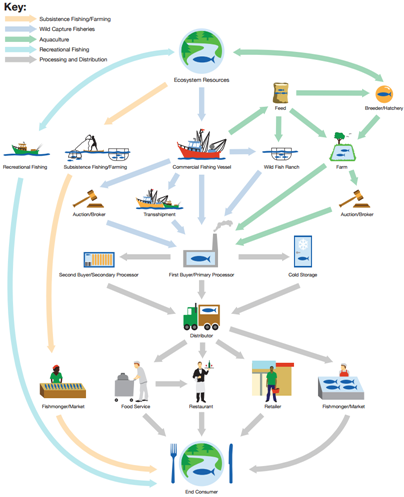
\includegraphics[scale=1.0]{figures/FishSupplyChain.png} \
   \caption{Source: \url{https://www.fishwise.org/images/fishwise_traceability_white_paper_august_2012.pdf}}
  \label{fig:supplychain}
\end{figure}

The supply chain through which fish are delivered is extremely complex (see Figure~\ref{fig:supplychain})
and involves diverse industries and regulatory controls that cross national boundaries. The
diversity of participants in the supply chain and the complex relationships between them makes this
a perfect opportunity of the use of blockchain technologies. A team at Intel is using the
Hyperledger Sawtooth blockchain technology to build a traceability prototype that combines the
distributed ledger, IoT sensors, and advanced communication technology to track telemetry parameters
such as location, temperature and humidity throughout capture, processing, and transit. Sensors
attached to the fish when it is caught record ownership and information about the location of the
catch in the ledger. Transactions on the ledger reflect interesting events in the processing of the
fish: ownership changes, transportation company, storage temperature range, etc. Further, analytics
on the ledger can be used for both regulatory enforcement and for scientific analysis of fish
harvesting and consumption.

The prototype highlights the benefits of Hyperledger Sawtooth as a platform for asset
traceability. The lightweight, highly decentralized consensus protocol in Sawtooth (``proof of
elapsed time'') is particularly well suited to the diverse, physically and organizationally
distributed ecosystem where potentially thousands of validating nodes are required. Broad
participation in the ledger reflects the cross-industry nature of the supply chain. Additionally,
asset tracking brings in a number of issues not generally seen in ledgers that focus on financial
products. For example, asset tracking requires handling of diverse data types such as the composite
format required for telemetry and environmental sensing. Transaction families in Sawtooth
accommodate domain-specific data and the transactions that operate on it, including enforcement of
data specific constraints (such as verification of the calibration of a sensor)

The use of blockchain technologies provides a number of benefits for cross-industry
traceability. Most importantly, blockchain technologies provide a means of establishing a public (to
the community of participants) and authoritative record of provenance. Its decentralized nature and
resiliency to faults enable updates from fishing boats, trucks, cold storage facilities and
restaurants. Beyond traceability, the digitization of assets (fish in this case) opens the doors for
completely new markets that might include, for example, monetization of provenance.
